Having set up the basic routing toolkit needed to construct a calendar being more intelligent than a standard one, this chapter wants to give details on this additional "intelligence". A calendar in this context is defined to be a list of events and tasks. A calendar is broken into pieces by default covering one day. Although it may in principle cover any period of time, it will be called \emph{day plan}.

\subsubsection{Representation of a day plan (\texttt{DayPlan} class)}

The \texttt{DayPlan} class is a container for events and tasks in the previously explained sense including functionality to operate on its content. Its core component is an algorithm to check whether any arbitrary event in the day plan is compliant with the assumption of "standing" at a fixed but arbitrary location at a fixed but arbitrary time\footnote{the considered event of course has to have a fixed location and start time}. This compliance furthermore depends on the (estimated) existence of the possibility to use a given vehicle to reach the considered event in time.\newline

A compliance check actually tries to find a route starting from the given location to the location of the considered event and returns the time left between the specified time and the start time of the considered event substracted by the estimated time needed to travers the calculated route. Since location and time to start and the event to consider as a target event are free parameters, this algorithm can be used in many ways to be the basis of every use-case.\newline

TODO: where do events and tasks come from?

\subsubsection{Compliance with current position and time}
 
One question our application is expected to give answer to is \emph{"How much time is left until I have to get going towards my next event to be there in time?"}.\newline

The answer is given by passing the current location (probably the last known GPS location) and the current time to the appropriate method of a \texttt{DayPlan} instance. By definition, the result is the answer to the question, with a negative value indicating an incompliance between the current position and the next event. Thus it can probably not be reached in time. Figure \ref{fig:compliance_check} gives a simplified graphical representation.

\begin{figure}[h!]
	\centering
	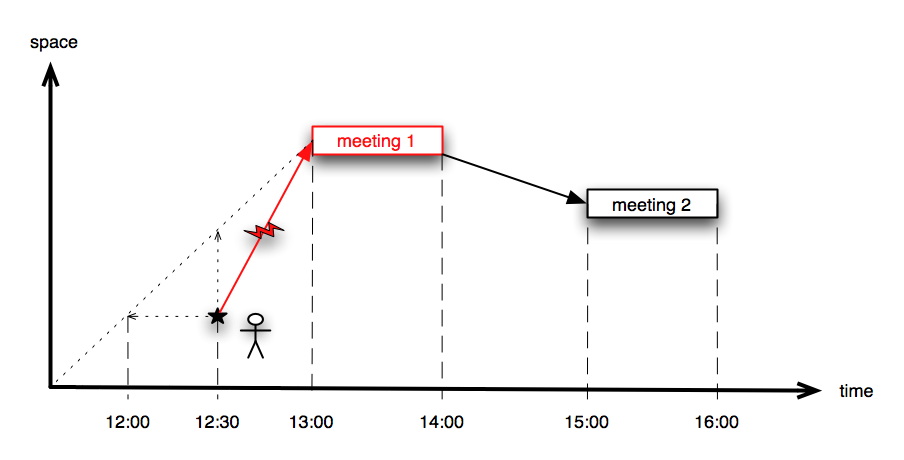
\includegraphics[width=15cm]{pics/compliance_check.png}
	\caption{A conflict revealed by a compliance check: The current position (marked with a stickman) is incompatible with the next event ("meeting 1") since the time neede to get there exceeds the time left. Space is reduced to one dimension for simplicity.}
	\label{fig:compliance_check}
\end{figure}

TODO: (Alex) some words on notifications

\subsubsection{Consistency check}

As a day plan probably contains more than one event, it bears potential for inconsistencies in the sense that at least one event cannot be reached in time\footnote{using one single specified vehicle} assuming one adheres to the previous event as fixed in the day plan. The user probably longs to be informed about such inconsistencies.\newline

A consistency check of a day plan is performed by iteratively checking compliance between one event and its preceeding event and returning a list of conflicts. A conflict can either simply be an incompliance between two subsequent events or any other conflict, including an incapability of finding a route or a temporal overlap between two events.











